%%
%% Author: Dario Chinelli
%% begin 2019-12-04
%% last mod 2022-02-02
%%

% Preamble
\documentclass[class=article, crop=false]{standalone}

% Packages
\usepackage[subpreambles=true]{standalone}
\usepackage{import}
\usepackage{graphicx}
\usepackage{amsmath}

% Document
\begin{document}
The recording technique employed to make this work possible is the Xovis sensor.
The entire field of view is covered using multiple cameras working together.
Starting from the raw images, each object is tracked down along its entire path.
This is possible using imaging recognition software.
The software give as output a data collection with coordinates and time for each pedestrian.

% \subsection{Kinect sensor: depth map based pedestrian tracking}

\subsection{Xovis 3D sensor}  % BIBLIO: www.xovis.com
The sensor is designed by \emph{Xovis company} and it is composed by two cameras that generate a stereo view.
The Xovis 3D sensors master every people counting and people flow measurement challenge with high precision. 
This technology enables people counting and tracking in real-time. 
Simple design, smart functionality and embedded processing build the base of our Xovis sensors. 
AI-based algorithms further improve the accuracy and flexibility of people counting and people flow management.
The signature 3D stereo vision technology permits accurate people counting of up to 99.9\%. 
Field-tested and proven for over a decade, these sensors stay true to Swiss precision.
The Xovis 3D stereo vision sensor with a powerful on-sensor person tracking engine always guarantees data privacy. 
Data is only transmitted in text format and without any kind of personally identifiable information. 
The sensors can be configured to be GDPR compliant.
Sensors can work together as one, covering large areas easily and tracking visitor paths.
\begin{figure}[h]
    \centering
    \subfloat[]{
        % \label{LABEL_1}
        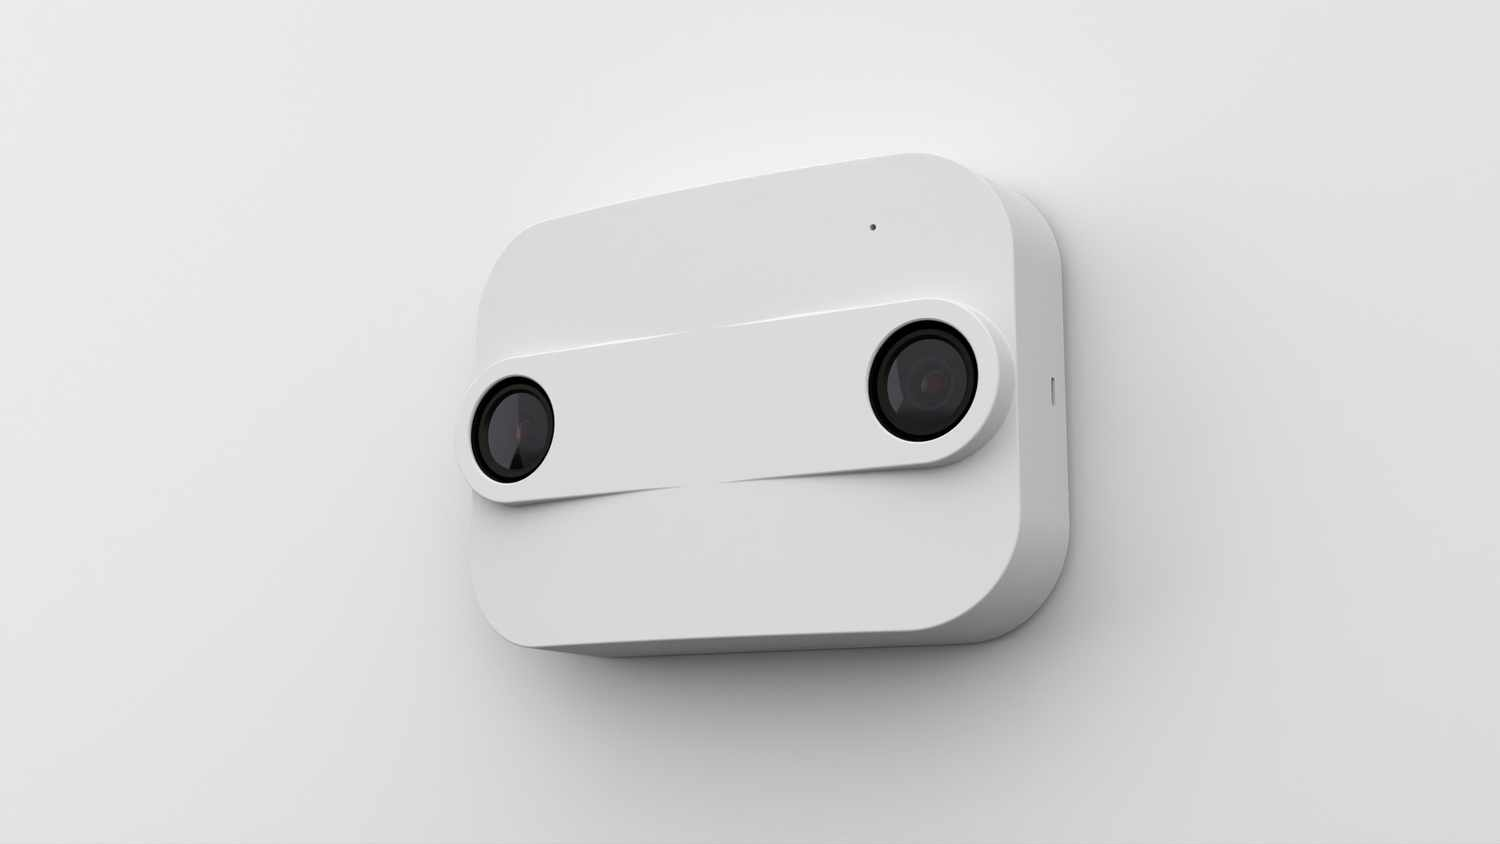
\includegraphics[ width=0.4\textwidth]{imgs/csm_PC2_CloseUp_Cam01_b6e9c5e401}
    }\quad\quad
    \subfloat[]{
        % \label{LABEL_2}
        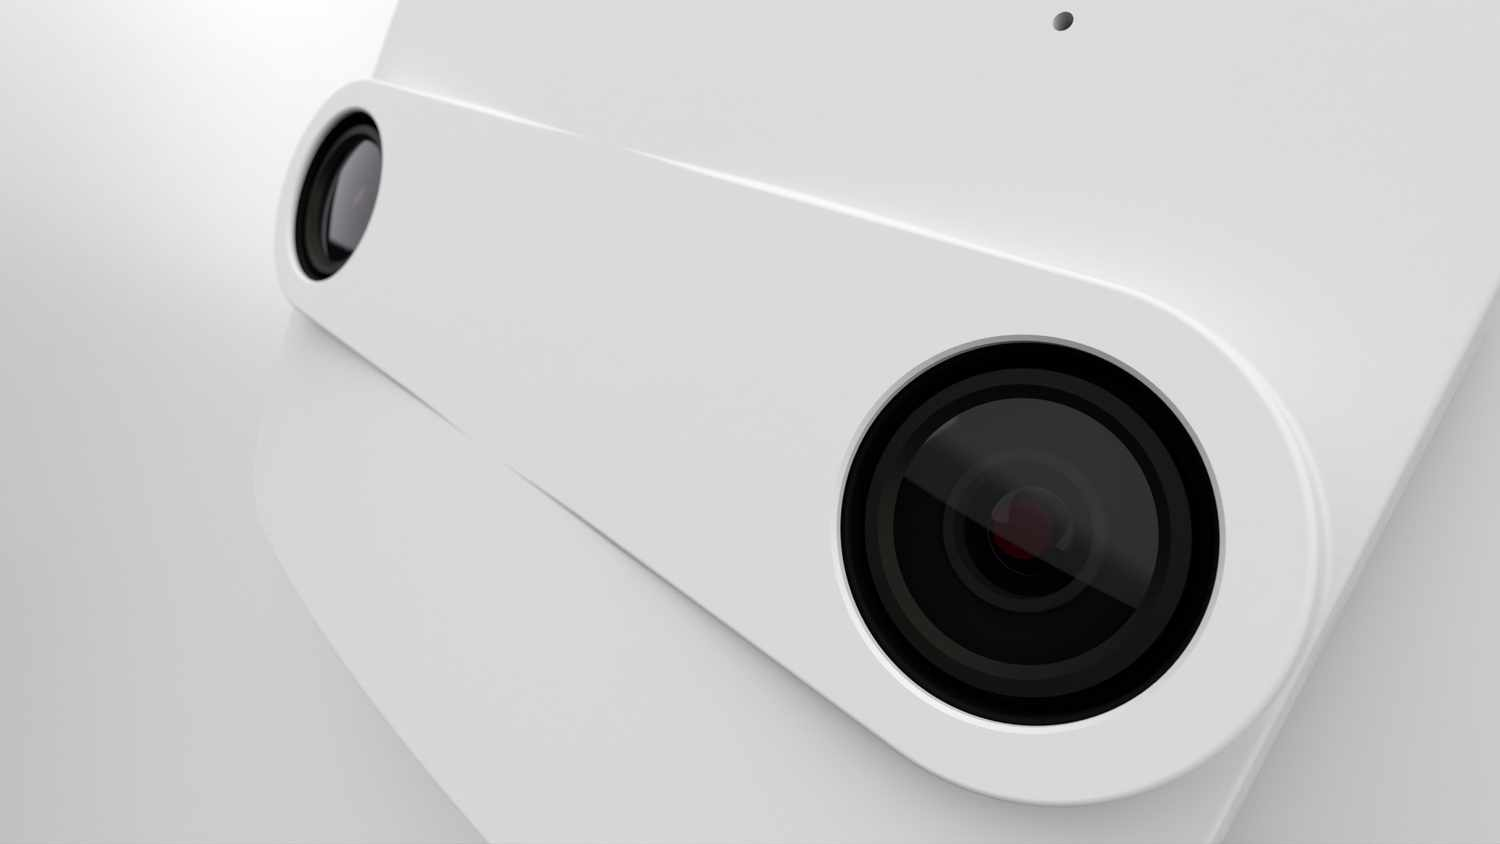
\includegraphics[ width=0.4\textwidth]{imgs/csm_PC2_CloseUp_Cam03_ad57a54722}
    }
    \caption{The Xovis 3D sensor.}
    \label{fig:Xovis_sensor}
\end{figure}

 

\end{document}
